% =====================================================================
%  main.tex —— 汇总文件（Lead 独占，队友不要修改）
%  Scott A. Wolpert, arXiv:1108.0174v1 —— 中文译注本
%
%  编译（本机）：powershell -ExecutionPolicy Bypass -File build.ps1
%  （LuaLaTeX，三遍；TMP 必须指向可写目录；镜像到 ASCII 目录编译）
% =====================================================================
% =====================================================================
%  Scott A. Wolpert,
%  "Lectures and notes: Mirzakhani's volume recursion and approach for the
%   Witten-Kontsevich theorem on moduli tautological intersection numbers"
%  arXiv:1108.0174v1 [math.DG] (31 Jul 2011) —— 中文译注本
%
%  编译：LuaLaTeX（本机 xdvipdfmx 不稳定，统一用 lualatex，编译 3 遍）
%  用法：powershell -ExecutionPolicy Bypass -File build.ps1
%
%  本底本的特殊性（译者必读）：
%   * 原文的**编号公式只有 4 条**：(1)(2)(3) 在 p.18，(4) 在 p.21；正文引用了它们（"formula (1)"、
%     "formulas (3)"）。这 4 条必须用 plain TeX 的 \eqno{(N)} 手工复刻编号，写法：
%         \[ H(x,y)=... \eqno{(1)} \]
%     两行共用一个编号时用 \[ \begin{aligned} ... \end{aligned} \eqno{(2)} \]。
%     其余公式**一律不编号**，禁止 \tag 与带编号的 equation/align。
%   * 原文的编号对象是**定理类陈述**：Theorem 1--15（其中 12 号是 Definition），
%     编号在全书连续，必须手工复刻（\begin{thm}{N}）。这是本项目的验收锚点。
%   * 图 1--11 为原文矢量图 500 dpi 截取（0 位图），图注为译者所译。
%   * % [Tutor Note: ...] 为译者批注，不进入排版，汇总见 译注汇总.md。
% =====================================================================
\documentclass[11pt,a4paper]{article}

\usepackage[UTF8]{ctex}
\usepackage{amsmath,amssymb,amsthm,mathtools}
\usepackage{bm}
\usepackage{graphicx}
\usepackage[a4paper,left=2.5cm,right=2.5cm,top=2.6cm,bottom=2.7cm]{geometry}
\usepackage[dvipsnames]{xcolor}
\usepackage{enumitem}
\usepackage{booktabs}
\usepackage{array}
\usepackage{multirow}
\usepackage{longtable}
\usepackage{multicol}
\usepackage{fancyhdr}
\usepackage{caption}
\usepackage{tcolorbox}
\usepackage{tikz}
\usepackage[hidelinks,unicode]{hyperref}
\hypersetup{pdftitle={讲义与注记：Mirzakhani 的体积递推与 Witten–Kontsevich 定理（中译注本）},
  pdfauthor={Scott A. Wolpert; 中译/批注: 本译本}}

\captionsetup{font=small,labelsep=quad}
\setlength{\emergencystretch}{3em}
\allowdisplaybreaks[1]
\graphicspath{{figures/}{../figures/}}

% ---------- 页眉 ----------
\pagestyle{fancy}
\fancyhf{}
\fancyhead[L]{\small\itshape Mirzakhani's volume recursion \& Witten-Kontsevich}
\fancyhead[R]{\small\thepage}
\renewcommand{\headrulewidth}{0.4pt}

% ---------- 定理类环境：编号一律由原文手工给出（原文 1--15 连续编号） ----------
% 用法：\begin{thm}{3} ... \end{thm}  /  \begin{prop}{11} / \begin{defn}{12} / \begin{cor}{N}
\newenvironment{thm}[1]{\par\medskip\noindent\textbf{定理 #1.}\ }{\par\medskip}
\newenvironment{prop}[1]{\par\medskip\noindent\textbf{命题 #1.}\ }{\par\medskip}
\newenvironment{defn}[1]{\par\medskip\noindent\textbf{定义 #1.}\ }{\par\medskip}
\newenvironment{corl}[1]{\par\medskip\noindent\textbf{推论 #1.}\ }{\par\medskip}
\newenvironment{lemmaenv}[1]{\par\medskip\noindent\textbf{引理 #1.}\ }{\par\medskip}

% 原文中不编号的 "Theorem." 段（如原文 p.3 的两条）——只有粗体标签、无编号
\newenvironment{thmplain}{\par\medskip\noindent\textbf{定理.}\ }{\par\medskip}
\newenvironment{thmplaincite}[1]{\par\medskip\noindent\textbf{定理.}\ [#1].\ }{\par\medskip}

% 原文 Proof. 环境
\renewcommand{\proofname}{证明}

% 原文的粗体/斜体行内小标题（如 "The papers." "First paper brief."）——
% 中文译为 \para{...}，独立成段、粗体、不缩进。
\newcommand{\para}[1]{\par\medskip\noindent\textbf{#1}\quad\ignorespaces}

% 原文图标题（手工编号，不用 \caption 自动编号）
\newcommand{\figtitle}[2]{\caption*{\small\textbf{图 #1：}#2}}
% 原文表标题（本项目底本 0 表，保留宏备用）
\newcommand{\tabtitle}[2]{\caption*{\small\textbf{表 #1：}#2}}

% 参考文献条目（Lead 手工转录，保留英文原貌）
\newcommand{\refitem}[2]{\par\hangindent=1.8em\hangafter=1\noindent [#1]~#2}

% 原文页码定位（批注/校对用；不进入排版）
\newcommand{\origp}[1]{}

% ---------- 常用记号（只能用这里定义过的宏，不要自造 \newcommand） ----------
\newcommand{\R}{\mathbb{R}}
\newcommand{\C}{\mathbb{C}}
\newcommand{\Z}{\mathbb{Z}}
\newcommand{\N}{\mathbb{N}}
\newcommand{\Q}{\mathbb{Q}}
\newcommand{\PP}{\mathbb{P}}
% 花体：模空间 M、Teichmüller T、曲线 C 等
\newcommand{\cA}{\mathcal{A}}
\newcommand{\cB}{\mathcal{B}}
\newcommand{\cC}{\mathcal{C}}
\newcommand{\cD}{\mathcal{D}}
\newcommand{\cE}{\mathcal{E}}
\newcommand{\cF}{\mathcal{F}}
\newcommand{\cG}{\mathcal{G}}
\newcommand{\cH}{\mathcal{H}}
\newcommand{\cI}{\mathcal{I}}
\newcommand{\cJ}{\mathcal{J}}
\newcommand{\cK}{\mathcal{K}}
\newcommand{\cL}{\mathcal{L}}
\newcommand{\cM}{\mathcal{M}}
\newcommand{\cN}{\mathcal{N}}
\newcommand{\cO}{\mathcal{O}}
\newcommand{\cP}{\mathcal{P}}
\newcommand{\cQ}{\mathcal{Q}}
\newcommand{\cR}{\mathcal{R}}
\newcommand{\cS}{\mathcal{S}}
\newcommand{\cT}{\mathcal{T}}
\newcommand{\cU}{\mathcal{U}}
\newcommand{\cV}{\mathcal{V}}
\newcommand{\cW}{\mathcal{W}}
\newcommand{\cX}{\mathcal{X}}
\newcommand{\cY}{\mathcal{Y}}
\newcommand{\cZ}{\mathcal{Z}}
% 本论文专用记号的简写
\newcommand{\T}{\mathcal{T}}                     % Teichmüller space（译者常用裸 \T）
\newcommand{\M}{\mathcal{M}}                     % moduli space（译者常用裸 \M）
\newcommand{\Tg}{\mathcal{T}_g}                 % Teichmüller space
\newcommand{\Tgn}{\mathcal{T}_{g,n}}
\newcommand{\Mg}{\mathcal{M}_g}                 % moduli space
\newcommand{\Mgn}{\mathcal{M}_{g,n}}
\newcommand{\cMgn}{\mathcal{M}_{g,n}}
\newcommand{\dimc}{\dim_{\C}}
\newcommand{\Mbar}{\overline{\mathcal{M}}}      % Deligne-Mumford 紧化
\newcommand{\Mgb}{\overline{\mathcal{M}}_g}
\newcommand{\Mgnb}{\overline{\mathcal{M}}_{g,n}}
\newcommand{\Tbar}{\overline{\mathcal{T}}}      % augmented Teichmüller space
\newcommand{\Tgnb}{\overline{\mathcal{T}}_{g,n}}
\newcommand{\MCG}{\mathrm{MCG}}                 % mapping class group
\newcommand{\WP}{\mathrm{WP}}                   % Weil-Petersson
\newcommand{\Vol}{\operatorname{Vol}}
\newcommand{\vol}{\operatorname{vol}}
\newcommand{\CV}{\operatorname{CV}}             % covolume
\newcommand{\Int}{\operatorname{Int}}
\newcommand{\Area}{\operatorname{Area}}
\newcommand{\len}{\ell}
\newcommand{\dl}{\mathrm{d}\ell}
\newcommand{\dtau}{\mathrm{d}\tau}
\newcommand{\dd}{\mathrm{d}}
\newcommand{\ee}{\mathrm{e}}
\newcommand{\ii}{\mathrm{i}}
\newcommand{\Tr}{\operatorname{Tr}}
\newcommand{\tr}{\operatorname{tr}}
\newcommand{\diag}{\operatorname{diag}}
\newcommand{\sgn}{\operatorname{sgn}}
\newcommand{\rk}{\operatorname{rk}}
\newcommand{\Res}{\operatorname{Res}}
\newcommand{\Id}{\mathrm{Id}}
\newcommand{\Stab}{\mathrm{Stab}}
\newcommand{\ie}{\textit{i.e.}}
\newcommand{\eg}{\textit{e.g.}}
\newcommand{\cf}{\textit{cf.}}
\newcommand{\half}{\tfrac{1}{2}}
\newcommand{\wt}[1]{\widetilde{#1}}
\newcommand{\what}[1]{\widehat{#1}}


\begin{document}

% =====================================================================
%  c00 —— 标题页、译者说明、目录（Lead 独占）
%  对应原文 PDF p.1（标题 / 作者 / 图 1 / 课程说明 / 脚注）
% =====================================================================

\begin{titlepage}
\centering
\vspace*{2.2cm}

{\Large\bfseries 讲义与注记\\[0.4em]
Mirzakhani 的体积递推，以及研究\\[0.1em]
模空间 tautological 相交数的\\[0.1em]
Witten--Kontsevich 定理的途径\par}

\vspace{1.6cm}
{\large Scott A. Wolpert\par}

\vspace{2.2cm}
{\normalsize 中文译注本\par}
\vspace{0.3cm}
{\small 底本：arXiv:1108.0174v1 [math.DG]，2011 年 7 月 31 日\par}
{\small （原文标题页另印有日期 November 27, 2024，为 PDF 生成日期，非论文发表日期；\par}
{\small 原文作者的资助脚注已移入下文"短课程说明"。）\par}
{\small 38 页 ／ 11 图 ／ 15 条编号陈述 ／ 33 条参考文献\par}

\vfill
{\small 译者说明与全部译者批注见《译注汇总》；编译方法与已知限制见《README》。\par}
\end{titlepage}

% [原文 p.1] —— 标题页附注：本材料是 2011 年 Park City 数学研究所研究生暑期学校
%  "Riemann 曲面模空间" 短课程的讲稿；作者致谢 Brad Safnuk 协助备课与授课；
%  作者受 NSF DMS-1005852 部分资助。
\section*{短课程说明（原文 p.1）}
\addcontentsline{toc}{section}{短课程说明（原文 p.1）}

本材料曾于 2011 年 Park City 数学研究所（Park City Mathematics Institute）研究生暑期学校
"Riemann 曲面模空间"（Moduli Spaces of Riemann Surfaces）的一门短课程中讲授。
Brad Safnuk 协助了课程的准备与运行；作者谨此感谢他的帮助。
（原文脚注：作者部分受美国国家科学基金会资助（Partially supported），批准号 DMS-1005852。）

% [原文 p.1] 图 1
\begin{figure}[htbp]
\centering
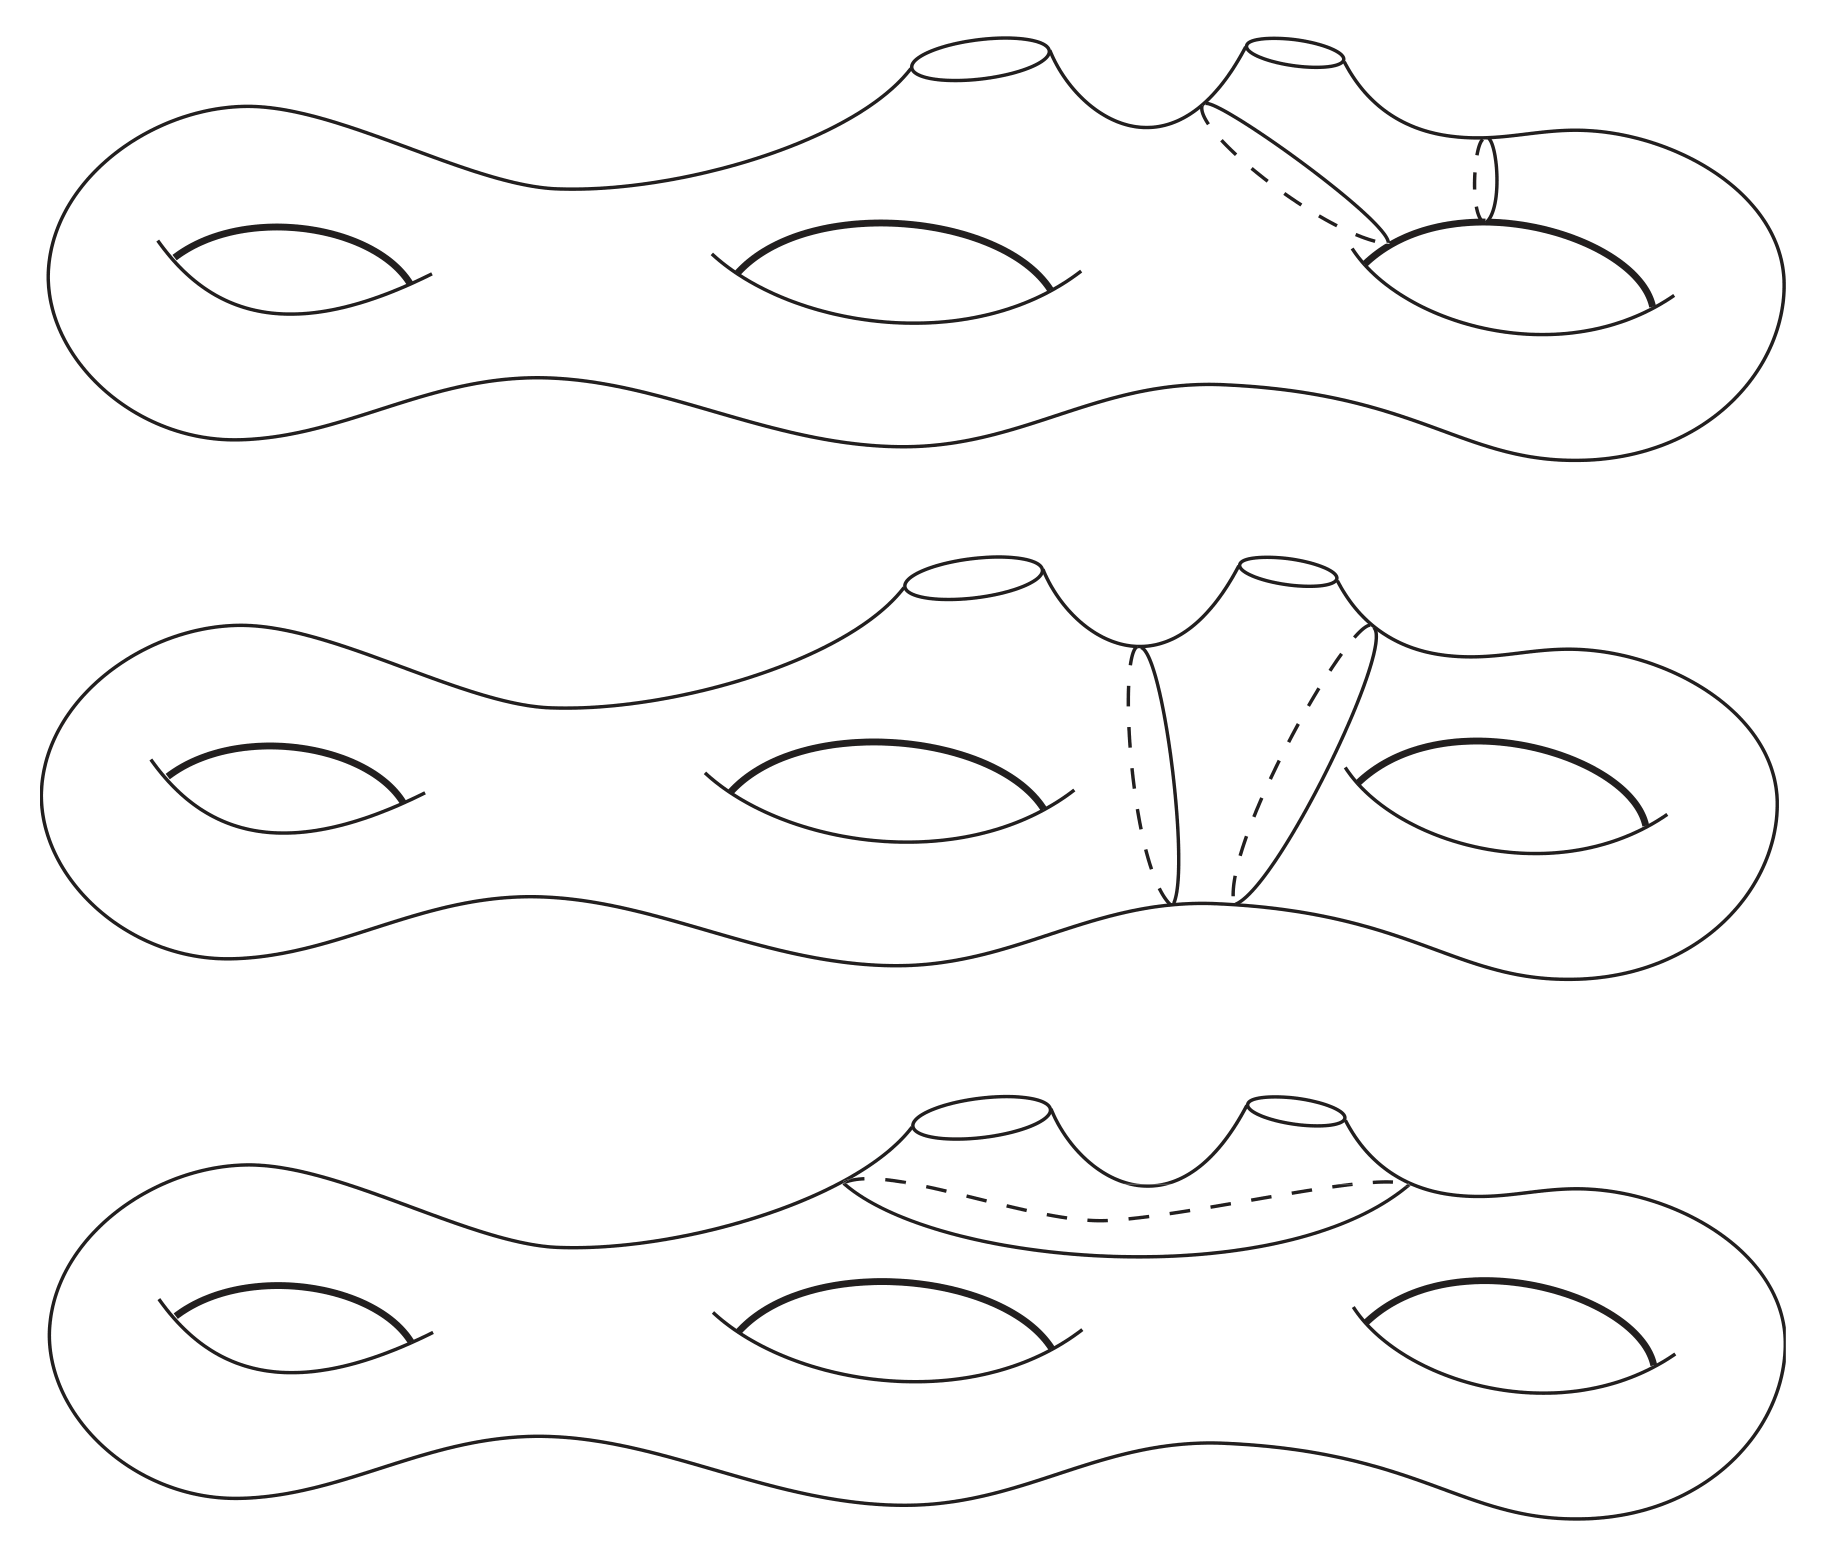
\includegraphics[width=0.62\textwidth]{fig01.png}
\figtitle{1}{长度恒等式所涉及的边界裤子构型。}
\end{figure}

% [Tutor Note: 图 1 画的是三条裤子（pants）在边界上按不同方式拼接得到的若干"边界裤子构型"，
%  与后文 §3 的长度恒等式 sum over pants 直接对应。读者若先记住"求和遍历所有嵌入的
%  β-裤子"，第 18--19 页的证明会顺畅得多。]

\vspace{1em}
\noindent\textbf{译者说明}\quad
（1）本译本以 2011 年 7 月 31 日 arXiv:1108.0174v1 为底本，全文 38 页。
底本的编号对象是 4 条编号公式（(1)--(4)）、15 条定理类陈述（Theorem 1--15，其中第 12 条为 Definition）
与 11 幅图，本译本逐一复刻其编号；其余公式底本未编号，译本同样不编号。

（2）正文严格照原文翻译，不放宽、不删节；凡解释性内容一律写入
\texttt{\% [Tutor Note: ...]} 注释，不进入排版。

（3）原文疑似的笔误照原样排，另行在批注中说明并给出正确形式（登记见 README）。

（4）参考文献保留英文原貌，逐条转录，未作翻译（学术惯例）。

\tableofcontents
\newpage
          % 标题页、译者说明、目录（Lead，原文 p.1）

% =====================================================================
%  c01 —— §1 引言（Lead 独占）
%  对应原文 PDF pp.2--3（印刷页码 2--3，偏移 0）
%  本节无编号陈述；p.3 的两条 "Theorem." 在原文中即为**不编号**的定理段，
%  用 thmplain 排版，切勿误编为 Theorem 1/2（编号 1 从 p.9 才开始）。
% =====================================================================

% [原文 p.2]
\section{引言}

\para{论文。}
\begin{itemize}[leftmargin=1.6em,itemsep=2pt,topsep=2pt]
\item \emph{Simple geodesics and Weil--Petersson volumes of moduli spaces of bordered
  Riemann surfaces.} Invent. Math., 167(1):179--222, 2007.
\item \emph{Weil--Petersson volumes and intersection theory on the moduli space of
  curves.} J. Amer. Math. Soc., 20(1):1--23, 2007.
\end{itemize}

% [Tutor Note: 这两篇（连同 [Mir08]）是 Mirzakhani 2014 年获 Fields 奖的三篇代表作。
%  第一篇解决"体积递推"，第二篇解决"系数是相交数"，第三篇（简单闭测地线计数）
%  把同一套体积递推用到计数问题上。下文 §3 的讲义主要按前两篇的顺序展开
%  （背景 → 长度恒等式 → 体积递推 → 辛约化与相交数 → Witten--Kontsevich）；
%  第三篇的计数结果不是 §3 的独立讲题。]

\para{论文的目标。}
\begin{enumerate}[leftmargin=1.8em,itemsep=2pt,topsep=2pt]
\item 导出 WP 模空间体积多项式的一条显式递推。
\item 应用辛约化，证明这些多项式的系数是相交数。
\item 证明该体积递推满足 Virasoro 关系——即 Witten 猜想。
\end{enumerate}

Maryam Mirzakhani 的这三篇论文 [Mir07a, Mir07b, Mir08] 之所以引人注目，
在于它们牵涉了大量高度发展的考量与内容。第一篇工作需要详细描述 Teichm\"uller 空间、
映射类群的作用、Weil--Petersson（WP）辛几何的公式、裤子（pair of pants）上简单
测地弧的分类、长度无穷和恒等式以及积分的精确计算。第二篇工作涉及模空间
tautological 类 $\kappa_1$ 与 $\psi$ 的描述（作为双曲几何中 $S^1$ 主丛的特征类）、
矩映射与精确的辛约化，以及组合计算。第三篇工作用到 Thurston 测度测地叶状结构
空间 $\cM\cG\cL$ 的分片线性（PL）结构、列车轨道（train-track）辛形式，以及 Masur
关于映射类群在 $\cM\cG\cL$ 上作用遍历的结果。这些工作的一个精彩之处在于，
它们展示了 Riemann／双曲曲面的几何、拓扑与形变理论的重要方面。三篇工作以及一篇
近期预印本都应用了 Mirzakhani 的体积递推。把 Mirzakhani 的工作放进 Witten--Kontsevich
理论的诸种研究途径中加以讨论，见 Mulase--Safnuk 论文 [MS08] 的第一节。Kontsevich
对 Witten 猜想的原始解法 [Kon92]（包括模空间上 tautological 类的基本几何与矩阵
积分的带状图展开）的简要阐述，见 Looijenga 的 Bourbaki 讨论班报告 [Loo93]。
Mirzakhani 体积递推、Witten--Kontsevich 的解法以及 WP 体积极限应用的简要阐述，
见 [Do11]。Mirzakhani 素简单测地线定理 [Mir08] 的整体性阐述，见 [Wlp10, 第 9、10 章]。
Mirzakhani 的工作只是这个高度活跃、研究者众多的学科的一部分；Google Scholar 显示
这三篇 Mirzakhani 论文被引用 200 次，而更一般地，Witten 关于二维引力与规范理论的
原始论文 [Wit91, Wit92] 被引用超过 1100 次。

% [Tutor Note: 原文 "Mirzakhani's prime simple geodesic theorem" 中的 "prime" 指
%  "素"（不可再分）的简单闭测地线，即在本原（primitive）意义下不可约的闭测地线，
%  不是"质数"。中译沿用"素简单测地线"这一约定。]

\para{第一篇论文简述。}
带边 Riemann／双曲曲面模空间覆盖的辛纤维积分解，与辛形式的
$\dd\ell\wedge\dd\tau$ 公式、以及测地长度和的一条万有恒等式相结合，
导出计算体积的一条显式递推。亏格 $g$、$n$ 条边界的曲面模空间的体积，
被证明是曲面边界长度的一个系数全正的多项式，其总次数为 $6g-6+2n$。

% [原文 p.3]
\para{第二篇论文简述。}
扭转 Hamilton 流与边界长度矩映射相结合，可对带边双曲曲面模空间族应用辛约化。
其推论是：体积多项式的系数是模空间的特征数。一个几何构造表明这些特征数就是
tautological 相交数。体积递推则被证明满足 Virasoro 代数约束。

下面的定理是这些论文最直接的结论。

% 原文 p.3 上两条 "Theorem." 均**不编号**
\begin{thmplain}
WP 体积多项式。体积多项式由总次数更小的体积多项式递推确定，
[Mir07a, 公式 (5.1) 与定理 8.1]。亏格 $g$、$n$ 条边界、边界长度为
$L=(L_1,\dots,L_n)$ 的双曲曲面的模空间，其体积 $V_{g,n}(L_1,\dots,L_n)$ 是多项式
\[
V_{g,n}(L)=\sum_{\substack{\alpha\\ |\alpha|\le 3g-3+n}} C_\alpha L^{2\alpha},
\]
其中 $\alpha=(\alpha_1,\dots,\alpha_n)$ 为多重指标，且 $C_\alpha>0$ 落在
$\pi^{6g-6+2n-2|\alpha|}\Q$ 中，[Mir07a, 定理 1.1 与 6.1]。其系数是相交数，由下式给出
\[
C_\alpha=\frac{2^{\delta_{1g}\delta_{1n}}}{2^{|\alpha|}\alpha!\,(3g-3+n-|\alpha|)!}
\int_{\Mgnb}\psi_1^{\alpha_1}\cdots\psi_n^{\alpha_n}\,\omega^{3g-3+n-|\alpha|},
\]
其中 $\psi_j$ 是沿第 $j$ 个穿刺点的余切线的 Chern 类，$\omega$ 是辛形式，
$\alpha!=\prod_{j=1}^n\alpha_j!$，而 $\delta_{**}$ 是 Kronecker 指示 delta，
[Mir07b, 定理 4.4]。
\end{thmplain}

% [Tutor Note: 这里 $L^{2\alpha}$ 是多重指标简写，指 $\prod_i L_i^{2\alpha_i}$。
%  分母中的 $2^{|\alpha|}\alpha!$ 不是 $\omega$ 归一化的产物：在最顶次 $|\alpha|=3g-3+n$
%  时被积式里根本没有 $\omega$（只有 $\int\psi^\alpha$），却仍带 $2^{|\alpha|}$，
%  所以它只能来自 $C_\alpha$ 与相交数 $\langle\tau^\alpha\rangle$ 之间的换算：
%  定理自身的定义给出 $(\alpha)_g=C_\alpha\,2^{-\delta_{1g}\delta_{1n}}
%  \prod_i\alpha_i!\,2^{|\alpha|}$，而在顶次
%  $(\alpha)_g=\langle\tau^{\alpha_1}\cdots\tau^{\alpha_n}\rangle_g=\int\psi^\alpha$（见 p.31），
%  故 $C_\alpha=2^{\delta_{1g}\delta_{1n}}\langle\tau^\alpha\rangle/(2^{|\alpha|}\alpha!)$。
%  （它与递归中双阶乘 $(2k+1)!!=(2k+1)!/(2^k k!)$ 的归一化一致，也可看作按矩映射变量
%  $L_j^2/2$ 展开体积的产物。）讲义取 $\omega=2\omega_{WP}=2\pi^2\kappa_1$
%  （p.4、p.6、p.10），这一条与 $2^{|\alpha|}$ 无关。
%  核对锚点：$(g,n)=(1,1)$ 时 $C_0=2\int_{\Mbar_{1,1}}\omega=2\cdot(\pi^2/12)=\pi^2/6$、
%  $C_1=\frac{2}{2}\int_{\Mbar_{1,1}}\psi=1/24$，与 $V_{1,1}=\pi^2/6+L^2/24$ 逐项吻合。]
%
% [Tutor Note: 原文写 $\delta_{**}$，这是"Kronecker 指示 delta"的缩写记法，
%  实指 $\delta_{1g}\delta_{1n}$（即只有 $(g,n)=(1,1)$ 时 $\delta_{**}=1$，其余为 0），
%  故公式在 $(1,1)$ 情形多出因子 $2$（注意不是 $1/2$）。它对应原文 p.20 的说明：
%  椭圆对合使椭圆情形的相交数乘 $1/2$（等价地，$V_{1,1}$ 按给定值的 $1/2$ 形式定义），
%  因此按"给定"体积写 $C_\alpha$ 时要在 $(1,1)$ 情形补回因子 $2$。]

\begin{thmplaincite}{Mir07a, 定理 6.3 与 6.4}
体积多项式首项系数的递推关系。对多重指标 $\alpha$，定义
\[
(\alpha_1,\dots,\alpha_n)_g=C_\alpha\times 2^{-\delta_{1g}\delta_{1n}}
\times\prod_{i=1}^n\alpha_i!\times 2^{|\alpha|},
\]
则当 $n>0$ 且 $\sum_i\alpha_i=3g-3+n$ 时，有 dilaton 方程
\[
(1,\alpha_1,\dots,\alpha_n)_g=(2g-2+n)(\alpha_1,\dots,\alpha_n)_g,
\]
而当 $n>0$ 且 $\sum_i\alpha_i=3g-2+n$ 时，有 string 方程
\[
(0,\alpha_1,\dots,\alpha_n)_g=\sum_{\alpha_i\neq 0}(\alpha_1,\dots,\alpha_i-1,\dots,\alpha_n)_g.
\]
\end{thmplaincite}

% [Tutor Note: 原文此处用圆括号 $(\alpha_1,\dots,\alpha_n)_g$ 而非 Witten 惯用的
%  尖括号 $\langle\tau_{\alpha_1}\cdots\tau_{\alpha_n}\rangle_g$。二者只在公式实际使用的
%  顶次情形（括号总次数 $=3g-3+$ 括号内指标个数）相等；对一般多重指标，圆括号是经
%  $C_\alpha$ 归一化后的系数记号。反例：$(g,n)=(1,1)$ 时 $(0)_1=\pi^2/12$，而
%  $\langle\tau_0\rangle_1=0$。本译本照原文保留圆括号（定义见原文 p.31 的
%  $\langle\tau_0^{d_0}\cdots\rangle_g$）。]
%
% [Tutor Note: "dilaton 方程"与"string 方程"是 Witten 猜想（KdV 层级）的两条基本约束，
%  名字来自二维引力的弦论解释：string 方程对应世界面度规的重参数化不变性（$L_{-1}$），
%  dilaton 方程对应伸缩变换（$L_0$）。这两条在原文 p.33 定理 14（[Mir07b, Theorem 6.1]，
%  $L_n(e^F)=0,\ n\ge-1$）中被统一为 $L_{-1}$、$L_0$ 两条约束；p.34 定理 15（[MS08]）
%  给出的是另一套算子 $V_k$ 的版本，勿与此混淆。]
          % §1 Introduction（Lead，原文 pp.2--3）

% ---- §2 组织纲要与阅读指南（原文 pp.4--7，tr-06）----
\InputIfFileExists{chunks/tr06a}{}{}

% ---- §3 讲义（原文 pp.8--35）----
\InputIfFileExists{chunks/tr01a}{}{}   % pp.8--9
\InputIfFileExists{chunks/tr01b}{}{}   % pp.10--11
\InputIfFileExists{chunks/tr01c}{}{}   % pp.12--13

\InputIfFileExists{chunks/tr02a}{}{}   % pp.14--15
\InputIfFileExists{chunks/tr02b}{}{}   % pp.16--17
\InputIfFileExists{chunks/tr02c}{}{}   % pp.18--19

\InputIfFileExists{chunks/tr03a}{}{}   % pp.20--21
\InputIfFileExists{chunks/tr03b}{}{}   % pp.22--23
\InputIfFileExists{chunks/tr03c}{}{}   % pp.24--25

\InputIfFileExists{chunks/tr04a}{}{}   % pp.26--27
\InputIfFileExists{chunks/tr04b}{}{}   % pp.28--29
\InputIfFileExists{chunks/tr04c}{}{}   % pp.30

\InputIfFileExists{chunks/tr05a}{}{}   % pp.31--32
\InputIfFileExists{chunks/tr05b}{}{}   % pp.33--34
\InputIfFileExists{chunks/tr05c}{}{}   % pp.35（含 References 标题）

% ---- 参考文献（原文 pp.35--38，保留英文原貌，tr-06 转录）----
\InputIfFileExists{chunks/c-refs}{}{}

\end{document}
